\section{Theoretische Grundlage}
\label{sec:Theorie}
Periodische Funktionen haben die Eigenschaft sich einerseits periodisch im Raum
\begin{equation}
  f(x + D) = f(x) \ ,
  \label{eqn:f(x)}
\end{equation}
als auch periodisch in der Zeit 
\begin{equation}
  f(t + T) =f(t)
  \label{eqn:f(t)}
\end{equation}
zu wiederholen. Dabei ist $T$ die Periodendauer und $D$ die Distanz nach dem sich ein Vorgang wiederholt. Solche Vorgänge lassen sich mittels der $2 \pi$ periodoschen Funktionen Sinus und Cosinus beschreiben, welche die Form 
\begin{eqnarray}
  f(t) = a sin \left( \frac{2 \pi}{T} t \right) \ ,	\\
  f(t) = a cos \left( \frac{2 \pi}{T} t \right)
  \label{eqn:sin}
\end{eqnarray}
haben. Mittels des Fouriersche Theorem lassen sich sämtliche sämtliche periodische Vorgänge in der Natur aus zusammensetzung mit der beiden Funktionen beschreiben.
\begin{equation}
  \frac{1}{2} a_0 + \sum^{\infty}_{n=1} \left( a_\text{n} cos n \frac{2 \pi}{T} t + b_\text{n} sin n \frac{2 \pi}{T} t \right) 
  \label{eqn:fourier}
\end{equation}
Vorraussetzung ist jedoch, dass die Reihe gleichmäßig konvergiert. Die Koeffizienten lassen sich nach
\begin{eqnarray}
  a_\text{n} = \frac{2}{T} \int^0_T f(t) cos n \frac{2 \pi}{T} t dt	\\
  b_\text{n} = \frac{2}{T} \int^0_T f(t) sin n \frac{2 \pi}{T} t dt
  \label{eqn:Koef}
\end{eqnarray}
berechnen. Dabei treten nur vielfache der $\nu_1$ Grundfrequenz auf, welche als harmonische Oberschwingung bezeichnet wird. Beim Auftragen der Amplitude gegen die Oberwellen ergibt sich ein Linienspektrum,
\begin{figure}
  \centering
  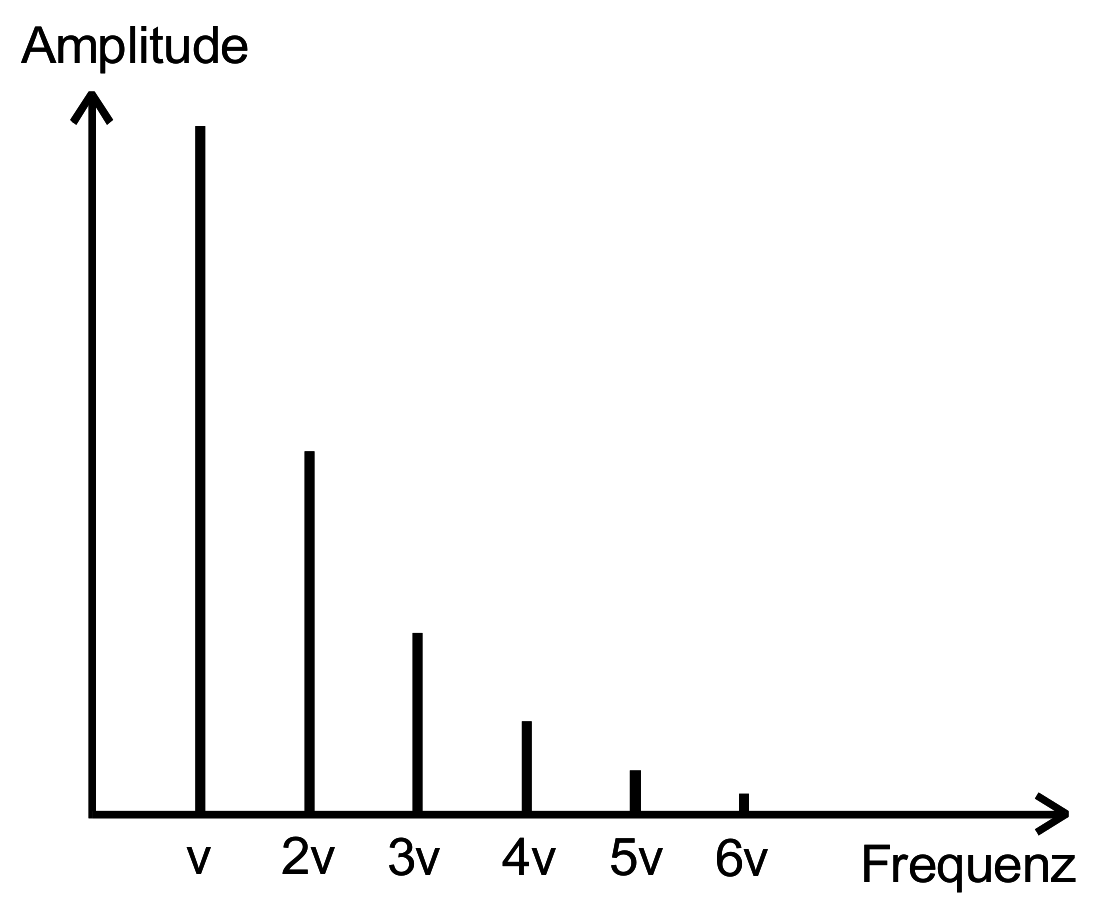
\includegraphics[height=4cm]{picture/Frequenzspektrum.png}
  \caption{Frequenzspektrum einer periodischen Schwingung}
  \label{fig:fre}
\end{figure}
bei welchen die Amplituden für n $\rightarrow \infty$ gegen null gehen sollte, wie man Abbildung \ref{fig:fre} entnehmen kann. Falls es sich bei der fourieranalysierten Funktion nicht um eine Periodische Funktion handeln sollte, ergibt sich dort ein kontinuierliches Spektrum.
Mit Hilfe der Fourier-Transformation ist es möglich das Frequenzspektrum sowohl periodischer als auch nicht-periodischer Funktion zu bestimmen. 
\begin{equation}
  g(\nu) = \int^{\infty}_{- \infty} f(t) e^{-i \nu t} dt
  \label{eqn:four-trafo}
\end{equation}
Da im Versuch nur über ein endlich langes Zeitintervall integriert werden kann, sind aufgrund der nicht periodizität Nebenmaxima zu erwarten. 
\subsection{Fehlerrechnung}
Sämtliche Fehlerrechnungen werden mit Hilfe von Python 3.4.3 durchgeführt.
\subsubsection{Mittelwert}
Der Mittelwert einer Messreihe $x_\text{1}, ... ,x_\text{n}$ lässt sich durch die Formel
\begin{equation}
	\overline{x} = \frac{1}{N} \sum_{\text{k}=1}^\text{N} x_k
	\label{eqn:ave}
\end{equation}
berechnen. Die Standardabweichung des Mittelwertes beträgt
\begin{equation}
	\Delta \overline{x} = \sqrt{ \frac{1}{N(N-1)} \sum_{\text{k}=1}^\text{N} (x_\text{k} - \overline{x})^2}
	\label{eqn:std}
\end{equation}

\subsubsection{Gauß'sche Fehlerfortpflanzung}
Wenn $x_\text{1}, ..., x_\text{n}$ fehlerbehaftete Messgrößen im weiteren Verlauf benutzt werden, wird der neue Fehler $\Delta f$ mit Hilfe der Gaußschen Fehlerfortpflanzung angegeben.
\begin{equation}
	\Delta f = \sqrt{\sum_{\text{k}=1}^\text{N} \left( \frac{ \partial f}{\partial x_\text{k}} \right) ^2 \cdot (\Delta x_\text{k})^2}
	\label{eqn:var}
\end{equation}

\subsubsection{Lineare Regression}
Die Steigung und y-Achsenabschnitt einer Ausgleichsgeraden werden gegebenfalls mittels Linearen Regression berechnet.
\begin{equation}
	y = m \cdot x + b
	\label{eqn:reg}
\end{equation}
\begin{equation}
	m = \frac{ \overline{xy} - \overline{x} \overline{y} } {\overline{x^2} - \overline{x}^2}
	\label{eqn:reg_m}
\end{equation}
\begin{equation}
	b = \frac{ \overline{x^2}\overline{y} - \overline{x} \, \overline{xy}} { \overline{x^2} - \overline{x}^2}
	\label{eqn:reg_b}
\end{equation}
